%
%  module_II.tex
%
%  Created by Drew Conway on 2010-05-24.
% 
%
\documentclass[xcolor=dvipsnames, 9pt]{beamer}

\newenvironment{code}{\begin{semiverbatim} \begin{footnotesize}}
{\end{footnotesize}\end{semiverbatim}}

\usepackage{graphicx}
\usepackage{amssymb}
\usepackage{amsfonts}
\usepackage{amsmath}
\usepackage{hyperref}
\usepackage{natbib}
\usepackage{color}
\usepackage{pdfsync}
\usepackage{chancery}
\usepackage{movie15}
\usepackage{pgfpages}
\usepackage{fancyvrb}
\usepackage{colortbl}
\usepackage{multirow}

% \definecolor{white}{rgb}{255,255,255}
% \definecolor{darkred}{rgb}{0.5,0,0}
% \definecolor{darkgreen}{rgb}{0,0.5,0}
% \definecolor{lightblue}{rgb}{0,0,0.7}

% \hypersetup{colorlinks,
%   linkcolor=white,
%   filecolor=darkred,
%   urlcolor=lightblue,
%   citecolor=darkblue}

\usepackage{beamerthemesplit}
\usetheme{Copenhagen}
\usecolortheme[named=Violet]{structure} 
\setbeamertemplate{navigation symbols}{}
\setbeamertemplate{itemize items}[triangle]
\setbeamertemplate{enumerate items}[default]
%\setbeameroption{show notes on second screen}
% \logo{
\includegraphics[width = 2cm]{../images/logos/500px-NYU_logo.png}}

\newcommand{\R}{\mathbb{R}}
\renewcommand{\d}{\mathsf{d}}
\newcommand{\dd}{\partial}
\newcommand{\E}{\mathsf{E}}
\newcommand{\bb}{\mathbf}

\title{Module II - Why do SNA in \texttt{NetworkX}}
\author{Drew Conway and Aric Hagberg}
% \institute{
\includegraphics[width = 4cm]{../images/logos/500px-NYU_logo.png}}
\date{June 29, 2010}

\begin{document} 

\begin{frame}[plain]
  \titlepage  
\end{frame}

\begin{frame}
	\frametitle{Agenda for Module II}
	Speed, Scalability \& Graph Types
	\begin{itemize}
	   \item Why speed and scalability matter
	   \item Comparing \texttt{NetworkX} to other SNA tools 
	   \item What can be a ``graph'' in \texttt{NetworkX}
	\end{itemize}
	\uncover<2->{How \texttt{NetworkX} complements Python's scientific computing suite
	\begin{itemize}
	   \item \texttt{SciPy}/\texttt{NumPy}
	   \item \texttt{Matplotlib}
	   \item GraphViz
	\end{itemize}}
	\uncover<3->{Getting data in and out of \texttt{NetworkX}
	\begin{itemize}
	   \item I/O basics
	   \item Pulling non-local data
	   \begin{itemize}
	       \item Directly from the web
	       \item External databases
	   \end{itemize}
	\end{itemize}}
\end{frame}

\section{Speed and scalability} % (fold)
\label{sec:speed_and_scalability}

\subsection{Network data size and tool scalabilty} % (fold)
\label{sub:network_data_size_and_tool_scalabilty}

\begin{frame}[fragile]
    \frametitle{Why should we worry about scalability?}
    The size of networks being studying has increased rapidly over the years...
    \begin{center}
        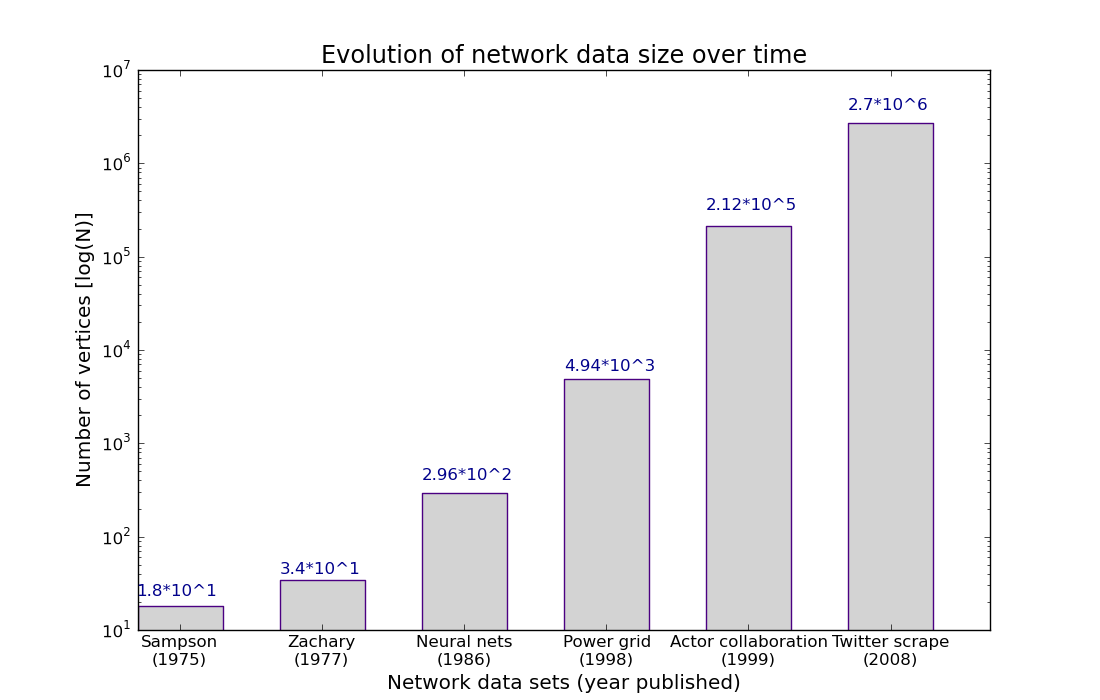
\includegraphics[scale=.35]{../images/figures/net_size_evo.png}
    \end{center}
    \uncover<2->{\alert{As network data becomes more readily available this trend will continue!}}
\end{frame}

\begin{frame}[fragile]
    \frametitle{How network size affects tools}
    While the data continues to scale up, many tools have not kept pace
    \begin{center}
        \begin{tabular}{clll}
            \multicolumn{4}{c}{\Large{Standard Network Analysis Tools}} \\ \hline\hline
            & \textbf{Tool} & \textbf{Base Algorithms} & \textbf{Platforms} \\ \hline
            \multirow{4}{*}{\textbf{Stand alone}} & UCINet & V=10K limit & Windows only \\
            & Pajek & V=100K limit & Windows only\\
            & ORA & C++/Java & Windows \& Linux \\
            & NetworkWorkbench & Java & Multi-platform \\ \hline
            \multirow{4}{*}{\textbf{Libraries}} & Statnet & R & Multi-platform \\
            & JUNG & Java & Multi-platform \\ 
            & \alert<2>{igraph} & \alert<2>{C/Fortran} & \alert<2>{Multi-platform} \\
            & \alert<2>{NetworkX} & \alert<2>{C/Fortran} & \alert<2>{Multi-platform}
        \end{tabular}
        \uncover<3->{\begin{columns}
            \column{.5\textwidth}
            \texttt{NetworkX} is designed to handle data sets of the scale being generated today
            \begin{itemize}
                \scriptsize{\item 10M's nodes and 100M's edges
                \item Read network data from local files, or from external sources
                \item Inherently multi-platform}
            \end{itemize}
            \column{.5\textwidth}
            \begin{center}
                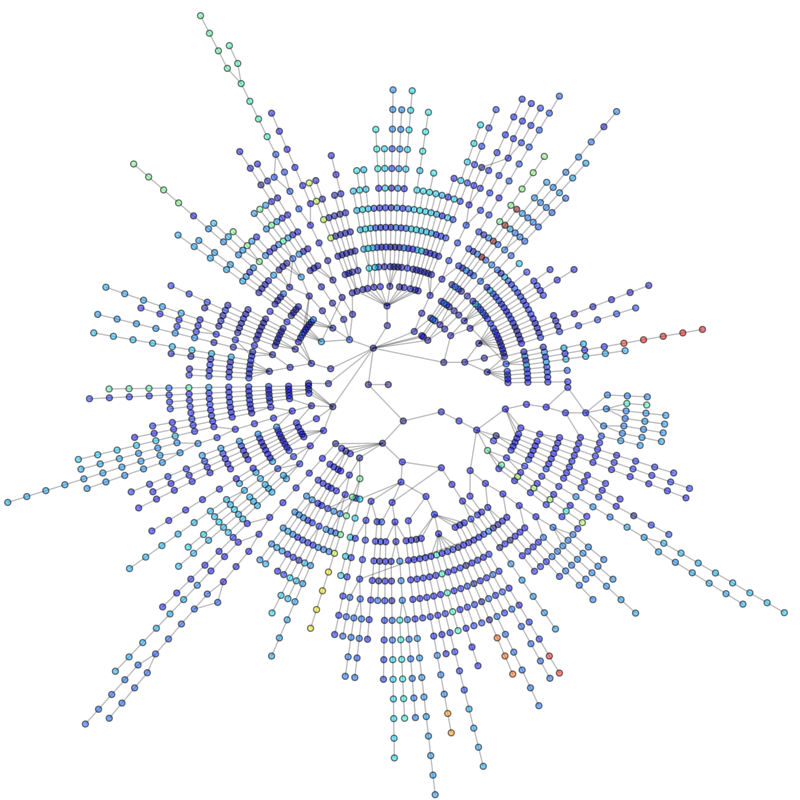
\includegraphics[clip,trim=4cm 4cm 4cm 4cm,width=2cm]{../images/networks/lanl_routes.png} \hspace{2mm}
                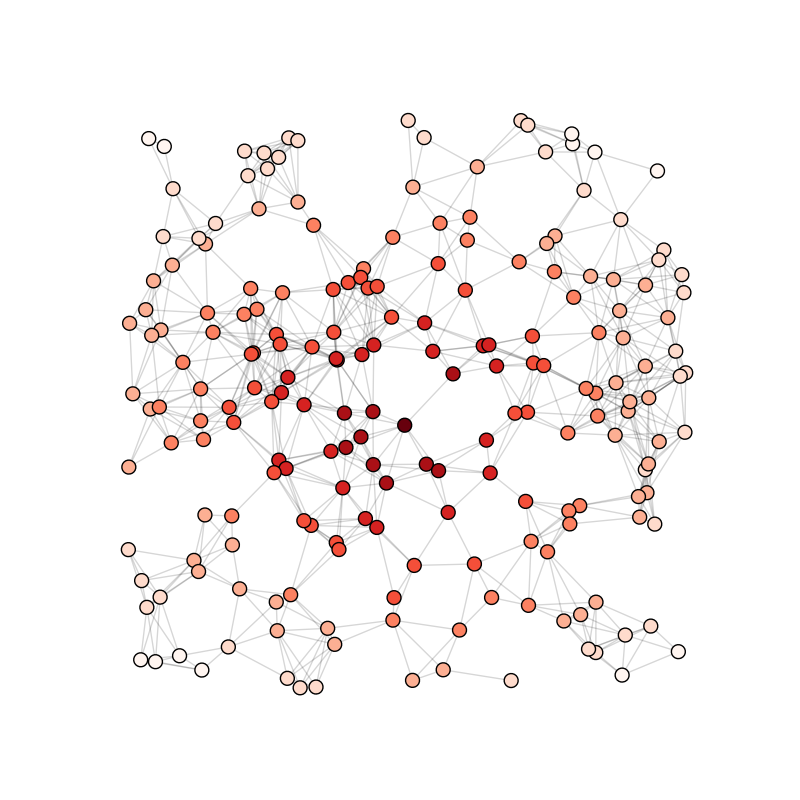
\includegraphics[clip,trim=4cm 4cm 4cm 4cm,width=2cm]{../images/networks/random_geometric_graph.png}
            \end{center}
        \end{columns}}
    \end{center}
\end{frame}

% subsection network_data_size_and_tool_scalabilty (end)

\subsection{Supporting non-traditional graph types} % (fold)
\label{sub:supporting_non_traditional_graph_types}

\begin{frame}[fragile]
    \frametitle{Moving beyond basic concepts of the ``graph''}
    In a more fundamental way, however, most network tools are limited in their concept of what can be a network
    \begin{itemize}
        \item Networks are collections of nodes and edges
        \item Nodes are static integers or strings, and edges are binary or continuous values
    \end{itemize}
    \texttt{NetworkX} can represent \textbf{ANY} relationship supported by Python data types
    \vspace{2mm}
    \begin{columns}
        \column{.3\textwidth}
        \small{Suppose we had data, or a data generating process, that was a time-series
        \begin{itemize}
            \item Current tools need kludges or hacks to add this data
            \item In \texttt{NetworkX}, we simply use the built-in Python \texttt{datetime} package to create a network of time-stamps
        \end{itemize}}
        \column{.7\textwidth}
        \begin{block}{}
            \begin{code}
\tiny{G=nx.DiGraph()
\alert<2>{# Create datetime object nodes
for v in xrange(num_nodes):
    G.add_node(datetime.now())
time_nodes=G.nodes()}
\alert<3>{# Add edges with `time' attribut
for i in xrange(num_nodes):
    draws=random.uniform(0,1,num_nodes)
    for j in xrange(num_nodes):
        if i!=j and draws[j]<=p:
            G.add_edge(time_nodes[i],time_nodes[j],time=datetime.now())
...}
\alert<4>{# target source datetime_created
2010-05-25 13:38:42.515323 2010-05-25 13:38:42.515492 
    \{`time': datetime.datetime(2010, 5, 25, 13, 38, 42, 515752)\}
...}}
                \end{code}
            \end{block}
    \end{columns}
\end{frame}

% subsection supporting_non_traditional_graph_types (end)

% section speed_and_scalability (end)

\section{Scientific computing in Python} % (fold)
\label{sec:scientific_computing_in_python}

\subsection{SciPy, NumPy and matplotlib} % (fold)
\label{sub:scipy_numpy_and_matplotlib}

\begin{frame}[fragile]
    \frametitle{Python's scientific computing holy trinity}
    \begin{columns}
        \column{.33\textwidth}
        \begin{center}
            \href{http://www.scipy.org}{
\includegraphics[width=3cm]{../images/logos/Scipylogo.png}}
        \end{center}
        \uncover<2->{Python's primary library for \textbf{mathematical and statistical} computing. Containing sub-libs for
        \begin{itemize}
            \item Numeric optimization
            \item Clustering
            \item Linear algebra
            \item ..and many others
        \end{itemize}}
        \uncover<3->{The primary data type in \texttt{SciPy} is an array
        \begin{itemize}
            \item Data manipulation is similar to that of MATLAB
        \end{itemize}}
        \vspace{3mm}
        \column{.33\textwidth}
        \begin{center}
            \href{http://numpy.scipy.org/}{
\includegraphics[clip,trim=0mm 2mm 0mm 2mm,width=2.5cm]{../images/logos/NumPy_logo.png}}
        \end{center}
        \uncover<4->{\texttt{NumPy} is an extension of the \texttt{SciPy} data type to include \textbf{multidimensional arrays and matrices}
        \begin{itemize}
            \item Provides many functions for working on arrays and matrices
            \item Very useful for representing relational data
        \end{itemize}}
        \uncover<5->{Both \textttt{SciPy} and \texttt{NumPy} rely on the C library \texttt{LAPACK} for very fast implementation}
        \column{.33\textwidth}
        \begin{center}
            \href{http://matplotlib.sourceforge.net/}{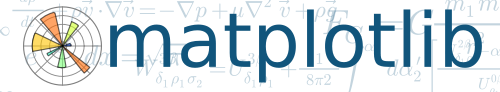
\includegraphics[width=3cm]{../images/logos/500px-Matplotlib_logo.png}}
        \end{center}
        \uncover<6->{\texttt{matplotlib} is \textbf{primary plotting library in Python}
        \begin{itemize}
            \item Supports 2- and 3-D plotting
            \item API allows embedding in apps
        \end{itemize}}
        \uncover<7->{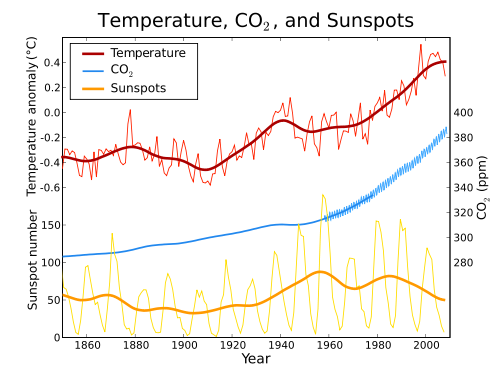
\includegraphics[width=2cm]{../images/figures/500px-Temp-sunspot-co2.png}
        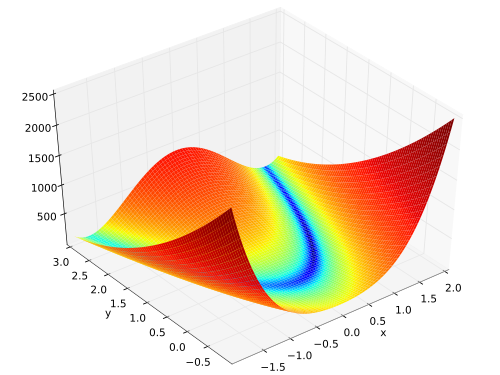
\includegraphics[width=2cm]{../images/figures/500px-Rosenbrock_function.png}}\\
        \uncover<8->{All graphics are highly customizable and professional publication ready}
    \end{columns}
    \vspace{1mm}
\end{frame}

% subsection scipy_numpy_and_matplotlib (end)

\subsection{Working with GraphViz} % (fold)
\label{sub:working_with_graphviz}

\begin{frame}[fragile]
    \frametitle{Exporting to GraphViz in \texttt{NetworkX}}
    \texttt{NetworkX} is designed to be an open-source all-purpose network manipulation and analysis tool
    \begin{itemize}
        \item Historically, the focus has not been on visualization
    \end{itemize}
    While there are several options for visualization in \texttt{NetworkX}, perhaps the best is its ability to read and write \texttt{GraphViz} files
    \begin{itemize}
        \item GraphViz is an open-source tool designed specifically for drawing graphs from the DOT language
        \item \texttt{NetworkX} works directly with GV using the \texttt{pygraphviz} package
    \end{itemize}
    \begin{columns}
        \column{.68\textwidth}
        \begin{block}{}
            \begin{code}
\tiny{\alert<2>{# Load Sampson monastery data from edgelist
>>> g2=nx.read_edgelist("samp_like_el.txt",create_using=nx.DiGraph())
>>> nx.info(g2)
Name:                  
Type:                  DiGraph
Number of nodes:       18
Number of edges:       55
Average in degree:     3.0556
Average out degree:    3.0556}
\alert<3>{# Convert to pygraphviz type
>>> g2_gv=nx.to_agraph(g2)}
\alert<4>{# Output DOT file and draw using dot layout
>>> g2_gv.write(``1samp_like_dot.dot'')
>>> g2_gv.draw(``samp_like.png'',prog=``dot'')}}
            \end{code}
        \end{block}
        \column{.32\textwidth}
        \begin{center}
            \uncover<5->{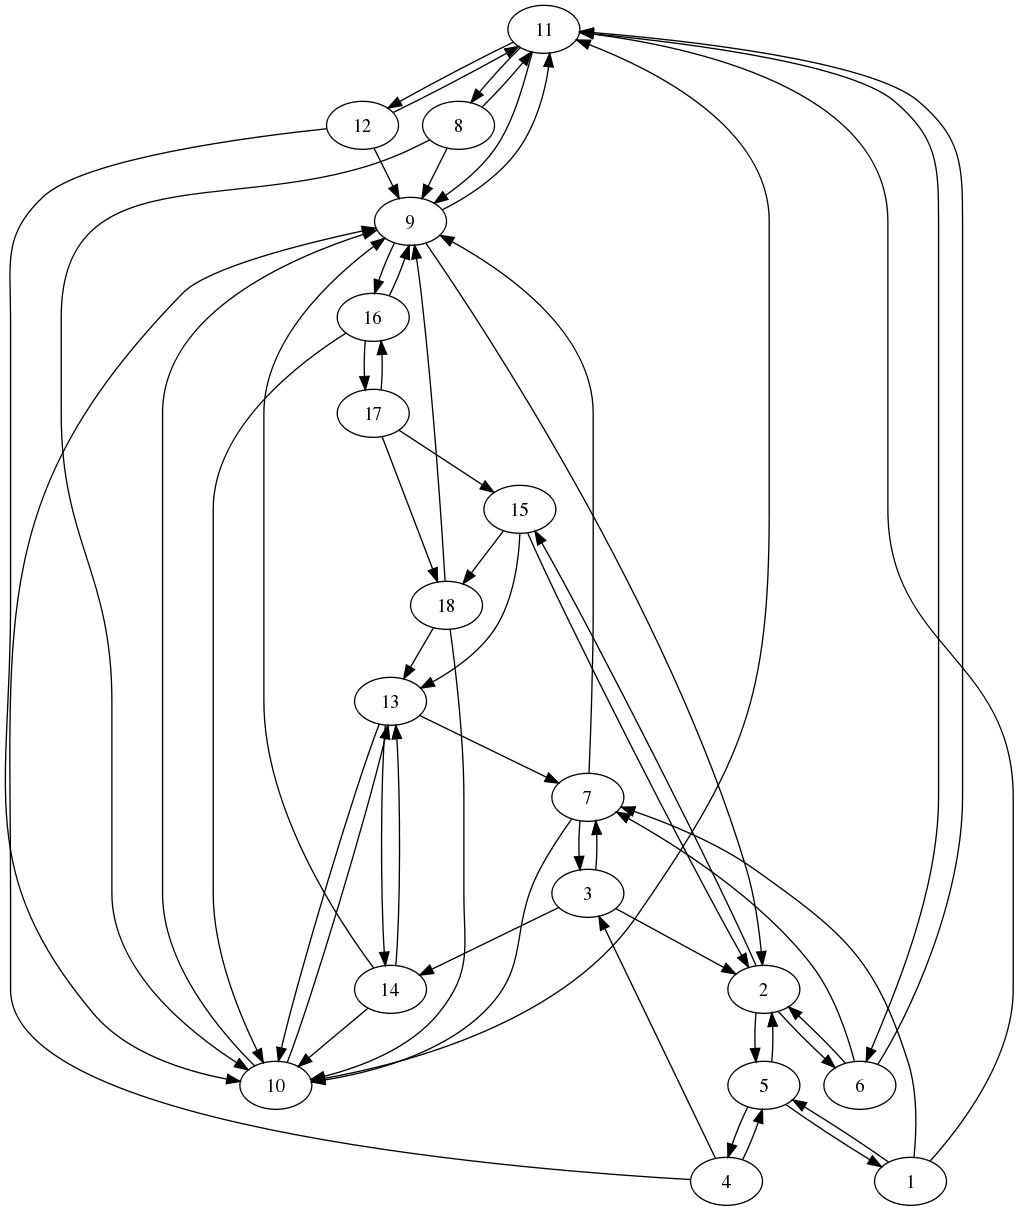
\includegraphics[height=4cm]{../images/networks/samp_like.png}}
        \end{center}
    \end{columns}
\end{frame}

% subsection working_with_graphviz (end)

% section scientific_computing_in_python (end)

\section{Data I/O from multiple sources} % (fold)
\label{sec:data_i_o_from_multiple_sources}

\subsection{Data I/O Basics} % (fold)
\label{sub:data_i_o_basics}

\begin{frame}[fragile]
    \frametitle{Getting local data into \texttt{NetworkX}}
    Getting data into \texttt{NetworkX} is as simple as a single line of code:
    \begin{block}{Loading local data file}
        \begin{code}
>>> G=read_edgelist("my_data.txt")
        \end{code}
    \end{block}
    \uncover<2->{Like many other network analysis platforms, \texttt{NetworkX} can parse a wide variety of network data types
    \begin{center}
        \begin{tabular}{cll}
            \multicolumn{3}{c}{\Large{Readable and Writeable Formats in NX}} \\ \hline \hline
            & \textbf{Format} & \textbf{Description} \\ \hline
            \multirow{3}{*}{\textbf{Standard}} & Edge list & 2 column, source\rightarrow target \\
            & Adjacency list & Each row 1st column as out-degree \\
            & Pajek & Edge list + node and edge attr \\ \hline
            \multirow{6}{*}{\textbf{Exotic}} & GML & Similar to DOT \\
            & GraphML & XML implementation \\
            & Pickle & Standard Python text output \\
            & LEDA & Between edge list and Pajek \\
            & YAML & Readable data serialization \\
            & SparseGraph6 & Adjacency list variant
        \end{tabular}
    \end{center}}
\end{frame}

% subsection data_i_o_basics (end)

\subsection{Loading data from external sources} % (fold)
\label{sub:loading_data_from_external_sources}

\begin{frame}[fragile]
    \frametitle{Network data available on the Internet}
    Recently, there has been an explosion of resources for scraping social graph
    \begin{table}
        \centering
        \scriptsize{
        \begin{tabular*}{.99\textwidth}{c|l|l}
        \textbf{Service} & \textbf{Data} & \textbf{API Docs} \\ \hline \hline
        
\includegraphics[height=4mm]{../images/logos/twitter_logo.png} & Following(ers), @-replies, date/time/geo & \url{http://apiwiki.twitter.com/} \\ \hline
        
\includegraphics[height=4mm]{../images/logos/facebook_logo.jpg} & Friends, Wall Posts, date/time & \url{http://developers.facebook.com/docs/api} \\ \hline
        
\includegraphics[height=4mm]{../images/logos/Newgooglelogo.png} & All SocialGraph relationships & \url{http://code.google.com/apis/socialgraph/} \\ \hline
        
\includegraphics[height=4mm]{../images/logos/foursquare.png} & Friends, Check-ins & \url{http://foursquare.com/developers/} \\ \hline
        
\includegraphics[height=3mm]{../images/logos/Hunch_com_logo.png} & ``Taste graph", recommendations  & \url{http://hunch.com/developers/} \\ \hline
        
\includegraphics[height=4mm]{../images/logos/nytlogo.png} & Congressional votes, campaign finance & \url{http://developer.nytimes.com/docs}
        \end{tabular*}}
    \end{table}
    \uncover<2->{There is clearly no shortage of data
    \begin{itemize}
        \item Each service provides different relational context
        \item Data formats are generally JSON, Atom, XML, or some combination
        \item Python has built-in parsers for all of these data types, which can easily be represented in \texttt{NetworkX}}
    \end{itemize}}
    \uncover<3->{\alert{Next, we will go over an example of building network data using Google's SocialGraph API}}
\end{frame}

\begin{frame}[fragile]
    \frametitle{Load data from databases}
    Along with the ability to parse data from online API's, NetworkX can create graphs from network data stored in various database formats
    \begin{itemize}
        \item All database platforms have either native or third-party libraries that allow read and write access from Python
    \end{itemize}
    \begin{center}
        \uncover<2->{\begin{tabular}{cll}
            \multicolumn{3}{c}{\Large{Ope-Source DB's Supported in Python}} \\ \hline \hline
            & \textbf{Database} & \textbf{Python Library} \\ \hline
            \multirow{3}{*}{\textbf{SQL}} & MySQL & MySQLdb \\
            & PosgreSQL & PyGreSQL \\
            & SQLite & sqlite3 \\ \hline
            \multirow{3}{*}{\textbf{NoSQL}} & Neo4j & Neo4j.py \\
            & MongoDB & PyMongo \\
            & CouchDB & couchdb-python 
        \end{tabular}}
    \end{center}
    \uncover<3->{\begin{itemize}
        \item This is just a small glance of all possible Python$\rightarrow$ DB bindings
    \end{itemize}}
\end{frame}

% subsection loading_data_from_external_sources (end)

% section data_i_o_from_multiple_sources (end)

\begin{frame}[plain]
    \frametitle{Module II Review}
    Why use \texttt{NetworkX} to do SNA?
    \begin{enumerate}
        \uncover<2->{\item Unlike many other tools, NX is designed to handle data on a scale relevant to modern problems}
        \uncover<3->{\item Most of the core algorithms in NX rely on extremely fast legacy code}
        \uncover<4->{\item Highly flexible graph implementations (a graph can be anything!)}
        \uncover<5->{\item Extensive set of native readable and writable formats}
        \uncover<6->{\item Takes advantage of Python's ability to pull data from the Internet or databases}
    \end{enumerate}
    \begin{center}
        \uncover<7>{\Huge{Questions?}}
    \end{center}
\end{frame}


\end{document}
